% CVPR 2027 submission, version 1.1 (2026-10-12). Teacher/student framing; devil's advocate terminology; teacher-uncertainty result.
\documentclass[10pt,twocolumn,letterpaper]{article}
\usepackage[review]{cvpr}
\usepackage{graphicx,booktabs,amsmath,amssymb,multirow,xcolor}
\usepackage{cuted,caption}
\definecolor{cvprblue}{rgb}{0.21,0.49,0.74}
\usepackage[pagebackref,breaklinks,colorlinks,allcolors=cvprblue]{hyperref}
\newcommand{\pend}[1]{{\color{red}[#1]}}
\def\paperID{*****}\def\confName{CVPR}\def\confYear{2027}
\title{Whoever Zooms Decides? Auditing the Evidence-Selection Interface\\of Gigapixel and High-Resolution Vision Models}
\author{Anonymous}
\begin{document}
\maketitle

\begin{abstract}
High-resolution vision systems rarely decide from the whole input. Multiple-instance learning (MIL) models classify gigapixel slides from a few attended patches, and ``thinking-with-images'' agents answer from the crops they zoom into. We audit this evidence-selection interface with controlled substitutions of \emph{authentic} regions: the image, features and answering model are fixed, and only the selected evidence changes, at a fixed inspection budget.
We find three distinct regimes. (i) \emph{Omission and override in MIL}: on CAMELYON16 an adversarial selector drives attention top-$B$ MIL from 0.97 to 0.00 balanced accuracy, and on BCNB realistic, non-adversarial selectors already change 9--61\% of slide decisions. Attacks on tumor slides succeed almost entirely by omitting every tumor witness, yet even a forced true witness is overridden by adversarially chosen authentic normal patches in 55--99\% of slides. (ii) \emph{Evidence-dependent VLM zoom}: for Qwen2.5-VL and Qwen3-VL on V* and HR-Bench, the model's own zoom is net helpful (it repairs 36--68\% of wrong answers and breaks 6--8\% of correct ones), but one adversarially chosen authentic crop breaks 38--57\% of correct answers. (iii) \emph{Tool insensitivity}: the RL-trained agent DeepEyes calls its zoom tool on every question, yet substituting the returned crop with the ground-truth, a random or an adversarial region changes 0--3\% of its answers, even on questions that require the crop.
We then ask whether \emph{competing} evidence acquisition makes a budget-restricted judge reliable, in the form of a clinical teaching round: two students who read the whole input argue assigned, opposite answers, and a teacher that sees only what they present decides. One student is always a devil's advocate. The teacher keeps 0.90--0.98 balanced accuracy on CAMELYON16 from a single tumor patch to 20\% tumor against greedy and look-ahead devil's advocates, while uniform random masking at the same budget is accurate only when evidence is dense. Matched-budget controls identify the effective ingredient: one-shot, class-conditioned counter-selection without alternation or presenter identity performs as well as debate, whereas two independent cooperative readers collapse when one is compromised. The teacher's own uncertainty is no substitute for the second student: a teacher shown only one side's evidence is confidently wrong and almost never asks for more. Under a fixed judge, competing acquisition tracks the \emph{number} of witnesses, while random masking tracks the hypergeometric probability of sampling one. A label-free variant in which every answer option has an advocate keeps VLM accuracy at the level of honest cooperative selection although all but one advocate argue for a wrong answer.
\end{abstract}

%=====================================================================
\section{Introduction}\label{sec:intro}
Gigapixel slides ($10^4$--$10^5$ patches) and 4K photographs exceed what a model processes at full resolution, so modern pipelines \emph{select}: an attention module keeps the top-scored patches~\cite{ilse2018abmil}, retrieval picks question-relevant regions~\cite{beacon2026}, or an agent calls a zoom tool and answers from the crop~\cite{wu2024vstar,zheng2025deepeyes}. Selection is the interface between image and decision, and it is usually evaluated only through end accuracy.

We audit that interface directly. Holding image, features and answerer fixed, we vary only \emph{which authentic regions} the answerer receives under a fixed inspection budget $B$, and we ask three questions. \textbf{Is the decision evidence-dependent?} If not, selection is neither useful nor a risk. \textbf{When it is, how does selection fail?} By omitting the diagnostic evidence, by showing authentic but misleading evidence that overrides it, or by a deployed reader that simply looks in the wrong place. \textbf{Can a restricted judge be protected} when it can only inspect $B$ items chosen by untrusted readers?

For the last question we borrow a structure from clinical teaching. In a case conference, residents who have studied the case present findings for competing diagnoses, and a senior physician who has not read the whole case questions them and decides; a devil's advocate is assigned to argue the less likely answer. The senior does not re-read the case, otherwise the residents would be unnecessary. We instantiate this as \emph{students} (cheap readers that see the whole slide or image) and a \emph{teacher} (the budget-restricted judge) that sees only the evidence the students present.

\paragraph{Contributions.}
\begin{itemize}
\item A \textbf{controlled substitution protocol} for selected-evidence systems with an explicit inspection budget, threat model and transition-level metrics (correct$\to$wrong and wrong$\to$correct, realized trajectory vs.\ best-of-candidates), applied to MIL on CAMELYON16 and BCNB and to VLM zoom on V* and HR-Bench (Sec.~\ref{sec:protocol}).
\item A \textbf{taxonomy of three regimes} with evidence for each (Sec.~\ref{sec:regimes}): override/omission in MIL, evidence-dependent but steerable VLM zoom, and tool insensitivity in an RL-trained zoom agent, whose robustness comes from ignoring the tool rather than using it well.
\item A \textbf{controlled evaluation of the teaching round} (competing evidence acquisition) for a budget-restricted teacher (Sec.~\ref{sec:defense}). Debate~\cite{irving2018debate}, static counter-selection, unflagged pooling and two independent readers are compared at equal budget with on-policy judges; the gain comes from \emph{class-conditioned counter-selection}, not from interaction. A fixed-judge sparsity grid shows it depends on witness count, not fraction, and an uncertainty-triggered teacher shows that doubt cannot detect omitted evidence: only an opposing student can.
\end{itemize}
We do not claim a new debate mechanism, worst-case soundness, or a compute saving: our readers inspect the whole input, and the judge's restriction is the deployment constraint we study (Sec.~\ref{sec:discussion}).

%=====================================================================
\section{Related work}\label{sec:related}
\paragraph{Selection in MIL.} BagShift~\cite{bagshift2026} introduced the paired protocol of changing only the patch selector for a fixed slide, features and predictor, for deployment selectors (tissue-wide vs.\ localized sampling at equal 128-patch budgets) on CAMELYON16 and PANDA, showing that localized views retain tumor in only 10\% of micrometastatic observations. We adopt this protocol and add adversarial, transferred and hypothesis-conditioned selectors, witness-retention analysis, VLM zoom agents and competing-acquisition defenses. Pixel-level attacks on MIL and pathology CNNs~\cite{mil_adv2022,foote2021now} perturb inputs rather than selection. Sufficiency methods (FOCI, GCE-MIL, ReaMIL, CAR-MIL)~\cite{foci2026,gcemil2026,reamil2026,carmil2026} ask which subsets suffice; BEACON~\cite{beacon2026} acquires evidence by expected information gain rather than relevance.
\paragraph{Zoom agents.} V*~\cite{wu2024vstar}, ViCrop~\cite{zhang2025vicrop}, DeepEyes~\cite{zheng2025deepeyes} and Mini-o3~\cite{minio3} answer from zoomed crops; ViEBench~\cite{viebench2026}, Pinpoint-Bench~\cite{pixeleyes2026} and Distract-Bench~\cite{distract2026} audit grounding without controlling the crop. MED~\cite{med2026} decomposes RL gains into intrinsic and tool-induced terms and finds limited tool-mediated correction; our crop-service substitutions are a complementary causal test of whether answers depend on the returned content.
\paragraph{Debate and prover--verifier games.} Debate with a sparse-pixel judge was proposed by Irving et al.~\cite{irving2018debate}, who also discuss gigapixel inputs. Merlin-Arthur classifiers~\cite{waldchen2024merlin} and the Neural Concept Verifier~\cite{ncv2026} analyse helpful and misleading selectors for a verifier; prover--verifier games~\cite{anil2021pvg,kirchner2024pvg,hammond2025nip} and LLM debate~\cite{khan2024debate,kenton2024scalable} study text. Multimodal debate has been used with a text-only judge~\cite{adhikari2025debating} and for deception monitoring~\cite{fang2026debateimages}. A public report found image-cell debate close to a random-mask ensemble~\cite{quantilized_debate}; we test whether evidence sparsity explains such outcomes, and which ingredient of debate matters.

%=====================================================================
\section{Protocol}\label{sec:protocol}
\paragraph{Selected-evidence decision and budget.} An input is a set of items $x=\{x_i\}_{i=1}^N$ (patches, or grid tiles at two scales). A selector returns a set $S\subseteq[N]$; a judge $J$ answers from $\{x_i\}_{i\in S}$, for VLMs together with a fixed $768^2$ global view. The \textbf{inspection budget} $B=|S|$ is the number of distinct items the judge sees. Every comparison in this paper is at equal $B$: in two-sided protocols each side contributes $B/2$ items. Random-mask ensembles use $M{=}32$ independent draws of $B$ items (32 judge calls, up to $32B$ exposures); we report them as a selector-free reference that receives \emph{more} judge inspection, not less.
\paragraph{Threat model.} The image and the judge are fixed and trusted to be what they are; the \emph{selector} is not. We distinguish: \textbf{deployed} selectors (the judge's own attention top-$B$; the VLM's own grounding zoom); \textbf{natural} selectors that a different but plausible pipeline would use (independent model attention, instance-classifier score, k-means coverage, question-relevance retrieval, hypothesis-confirming retrieval, confirmation zooms for each option); and \textbf{research attackers}: white-box greedy selection on exact judge logits toward a target answer, look-ahead (rollout) selection, black-box transfer from a surrogate model, and a \emph{constrained} attacker that must include a true witness. Attackers choose among authentic regions only; no pixels are modified. Natural and transfer selectors are implementable; white-box attackers measure worst-case interface susceptibility.
\paragraph{Metrics.} MIL: balanced accuracy (BA) and \emph{flip} = fraction of slides whose decision differs from the deployed selector's. VLM: we report transitions relative to the global-view answer, correct$\to$wrong (denominator: questions the global view answers correctly) and wrong$\to$correct, and we separate the \emph{realized} deployed trajectory (the model's own zoom) from \emph{best-of-candidates} stress tests over a selector family. 95\% bootstrap CIs over questions; MIL results are mean$\pm$sd over 3 seeds.
\paragraph{Teaching rounds: competing-acquisition protocols (all at budget $B$).} Students see every item; the teacher (judge) sees only presented items. Whenever a student is assigned the wrong answer it acts as a devil's advocate and argues that answer as strongly as it can, using authentic evidence only. \textbf{Debate}: two students are assigned opposite labels and alternately reveal $B/2$ items each, each move greedy on the judge's exact incremental logit given the transcript so far; the judge sees items plus a presenter flag (which side revealed it, not which side is honest); first mover random. \textbf{Static counter-selection}: each side selects $B/2$ items for its label without seeing the other side's items; union shown with flags. \textbf{Unflagged union}: as static, flags removed. \textbf{Two readers}: two independently trained attention readers contribute $B/2$ each (cooperative), or one is replaced by an adaptive adversary. Every protocol gets its own judge, trained on-policy from the same warm start for the same number of rounds. For VLMs, \textbf{label-free advocacy}: every answer option gets an advocate that reveals its best-supporting tile; the judge (the same VLM) sees the global view plus all advocates' tiles, labelled by the option they support, in random order. No ground-truth label is used. The binary MIL setting needs no label either: the two readers cover both classes.
\paragraph{Data and models.} CAMELYON16~\cite{c16} (UNI~\cite{uni} features; ResNet50 Barlow-Twins features (\texttt{resnet50\_bt}) distributed with the torchmil release as a second encoder\pend{verify: Kang et al.~\cite{kang2023benchmarking} pathology weights?}; 512px level-0 patches, 270/129 split, 49 tumor test slides, patch-level lesion labels); BCNB~\cite{bcnb} ER/PR/Grade-3 (CONCH~\cite{conch} features, 5-fold CV); V*-Bench~\cite{wu2024vstar} (191) and HR-Bench-4K~\cite{hrbench} (200, answer positions rotated); judges Qwen2.5-VL-7B~\cite{qwen25vl} and Qwen3-VL-8B~\cite{qwen3vl}; zoom agent DeepEyes-7B~\cite{zheng2025deepeyes} with its official tool protocol (generation stopped at \texttt{</tool\_call>} as in its RL environment). MIL judge: gated ABMIL~\cite{ilse2018abmil} with a presenter-flag input.

%=====================================================================
\section{Three regimes of selector failure}\label{sec:regimes}
\subsection{MIL: omission and override}
\begin{table}[t]\centering\small
\caption{\textbf{CAMELYON16} (BA, mean$\pm$sd over 3 seeds; full-slide ABMIL .969). $B$ = items inspected by the judge. Cooperative selectors are accurate but are driven to $\approx$0 by a white-box selector.}\label{tab:c16}
\setlength{\tabcolsep}{3pt}
\resizebox{\linewidth}{!}{\begin{tabular}{@{}lcccccc@{}}\toprule
$B$ & attn & attn (att.) & V-IP (att.) & cons. (att.) & rand-mask$^\ast$ & debate\\\midrule
2  & .974 & .021 & .000 & .000 & .556 & \textbf{.943}$\pm$.023\\
4  & .978 & .000 & .000 & .000 & .628 & \textbf{.949}$\pm$.010\\
8  & .984 & .000 & .000 & .000 & .628 & \textbf{.971}$\pm$.011\\
16 & .978 & .000 & .000 & .000 & .703 & \textbf{.958}$\pm$.008\\\bottomrule
\end{tabular}}\\[1pt]{\footnotesize $^\ast$32 random draws of $B$ items, mean logit.}
\end{table}

\begin{table}[t]\centering\small
\caption{\textbf{Realistic selectors already change MIL decisions} (BCNB-ER, ABMIL top-$B$ judge, $B{=}8$; flip relative to the deployed own-attention decision).}\label{tab:natural}
\begin{tabular}{@{}lcc@{}}\toprule
selector & BA & flip\\\midrule
own attention top-$B$ (deployed) & .758 & --\\
independent model's attention & .741 & .091\\
k-means coverage & .635 & .266\\
question-relevance retrieval & .613 & .177\\
confirm majority hypothesis & .525 & .232\\
confirm minority hypothesis & .581 & .608\\\midrule
black-box transfer (indep.\ full-slide surrogate) & .240 & .642\\
transfer from TransMIL surrogate & .110 & .681\\
white-box greedy & .020 & .784\\\bottomrule
\end{tabular}\end{table}

Tab.~\ref{tab:c16}: with slide, features and judge fixed, a white-box selector drives attention top-$B$, a V-IP querier~\cite{chattopadhyay2023vip} and a single adversarial consultant to $\approx$0 on CAMELYON16 at every budget. Selectors optimized against an independent surrogate transfer (BCNB-ER: .110--.240, Tab.~\ref{tab:natural}), and \emph{non-adversarial} selectors already change 9--61\% of decisions; seeking evidence for the minority hypothesis flips 61\%.

\textbf{Omission vs.\ override.} On tumor slides an attack can succeed by omitting every witness or by showing a witness together with authentic normal patches that outweigh it. For the attention top-$B$ judge (3 seeds), the unconstrained attacker flips 100\% of tumor slides and 98--100\% of these successes contain no tumor patch: the dominant failure is \emph{omission}. Forcing the most-attended true witness into the selection does not protect the judge: the attacker fills the remaining $B{-}1$ slots with authentic normal patches and still flips 99\% ($B{=}2$), 89\% ($B{=}4$) and 55$\pm$38\% ($B{=}8$) of tumor slides, so retained evidence is also \emph{overridden}. Normal-slide attacks (97--100\% success) are necessarily of this second kind: authentic normal tissue read as tumor.

\subsection{VLM zoom: evidence-dependent and steerable}
\begin{table}[t]\centering\small
\caption{\textbf{VLM zoom transitions} relative to the global-view answer (95\% bootstrap CI). Adversarial = best-of all grid tiles (white-box option scores); realized = the model's own grounding zoom.}\label{tab:vlm}
\setlength{\tabcolsep}{2.5pt}
\resizebox{\linewidth}{!}{\begin{tabular}{@{}lccc@{}}\toprule
 & V* Qwen2.5 & V* Qwen3 & HR-4K Qwen2.5\\\midrule
global-view acc & .665 & .691 & .600\\
full high-res acc & .707 & .743 & .590\\\midrule
\multicolumn{4}{@{}l}{\emph{correct$\to$wrong} (among global-correct)}\\
\ adversarial tile & .457 {\tiny[.37,.55]} & .568 {\tiny[.49,.65]} & .383 {\tiny[.30,.48]}\\
\ random tile (expected) & .092 & .130 & .132\\
\ best-of natural zooms & .087 & .073 & .192\\
\ realized own zoom & .063 & .058 & .080\\\midrule
\multicolumn{4}{@{}l}{\emph{wrong$\to$correct} (among global-wrong)}\\
\ realized own zoom & .590 & .675 & .359\\
\ some tile & .969 & .949 & .700\\\bottomrule
\end{tabular}}\end{table}

Tab.~\ref{tab:vlm}: the VLM's answer depends strongly on the crop. The deployed zoom is net helpful (it repairs 36--68\% of wrong answers and breaks 6--8\% of correct ones), and plausible alternative zooms are only mildly harmful (7--19\%). The risk is concentrated in adversarial choice: one authentic tile, shown together with the global view, breaks 38--57\% of correct answers, 3--5$\times$ the random-tile rate. The same evidence dependence that makes zoom useful (some tile repairs 70--97\% of wrong answers) makes it steerable.

\subsection{Tool insensitivity: an RL-trained zoom agent}
\begin{table}[t]\centering\small
\caption{\textbf{DeepEyes-7B crop-service substitution} (V*, 191 questions; every substitution replaces every crop the agent requests). Transitions relative to the agent's own rollout. Crop-necessary: questions Qwen2.5-VL answers wrongly from the global view but correctly with the GT tile (n=46).}\label{tab:deepeyes}
\setlength{\tabcolsep}{3pt}
\begin{tabular}{@{}lcc@{}}\toprule
overview given to the agent & full-res & 768$^2$\\\midrule
native accuracy (tool used on 100\%) & .832 & .681\\
GT crop: accuracy & .838 & .707\\
adversarial crop: correct$\to$wrong & .025 & .015\\
random crop: correct$\to$wrong & .006 & .015\\
blank crop: correct$\to$wrong & .013 & .030\\
crop from another image: correct$\to$wrong & .006 & .030\\
valid-box adversary: correct$\to$wrong & .006 & .007\\\midrule
crop-necessary: native & .696 & .239\\
crop-necessary: GT crop & .696 & .283\\\bottomrule
\end{tabular}\end{table}

DeepEyes~\cite{zheng2025deepeyes} calls its zoom tool on every question, but its answers barely depend on what the tool returns (Tab.~\ref{tab:deepeyes}). Replacing every returned crop with the ground-truth region raises accuracy by at most 2.6 points; adversarial, random, blank, and other-image crops all change at most 3\% of correct answers. On crop-necessary questions with a $768^2$ overview, where the answer is not resolvable from the overview, the agent stays at 24\% and the ground-truth crop lifts it only to 28\%. Transcripts assert that ``the zoom-in confirms'' the answer for crops that do not contain the object. This agent is robust to selection attacks because it does not use the selected evidence, a third regime distinct from robust evidence use, and consistent with MED~\cite{med2026}.

\begin{figure}[t]\centering
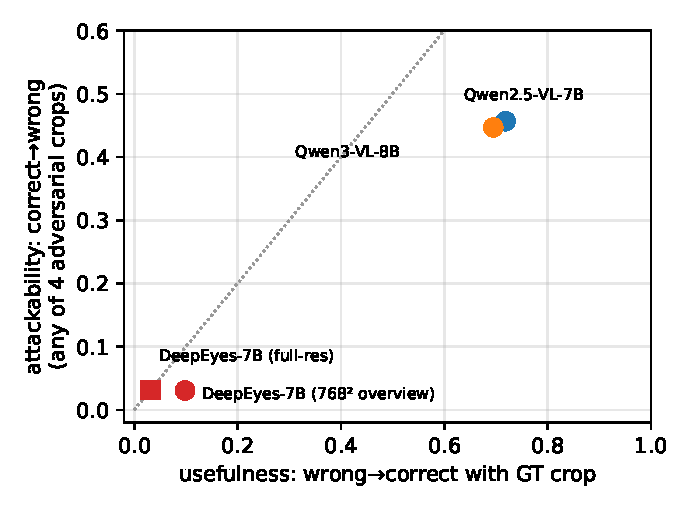
\includegraphics[width=0.92\linewidth]{figs/fig_useful_attack.pdf}
\caption{\textbf{Usefulness and attackability move together} (V*). x: wrong$\to$correct when the GT crop is supplied; y: correct$\to$wrong under any of the \emph{same} four crops chosen with a Qwen2.5-VL surrogate (for Qwen3-VL and DeepEyes this is a black-box transfer attack). Evidence-dependent zoom is both useful and steerable; DeepEyes is neither.}\label{fig:useful}
\end{figure}

%=====================================================================
\section{Can a teaching round protect a restricted teacher?}\label{sec:defense}
\begin{figure*}[t]\centering
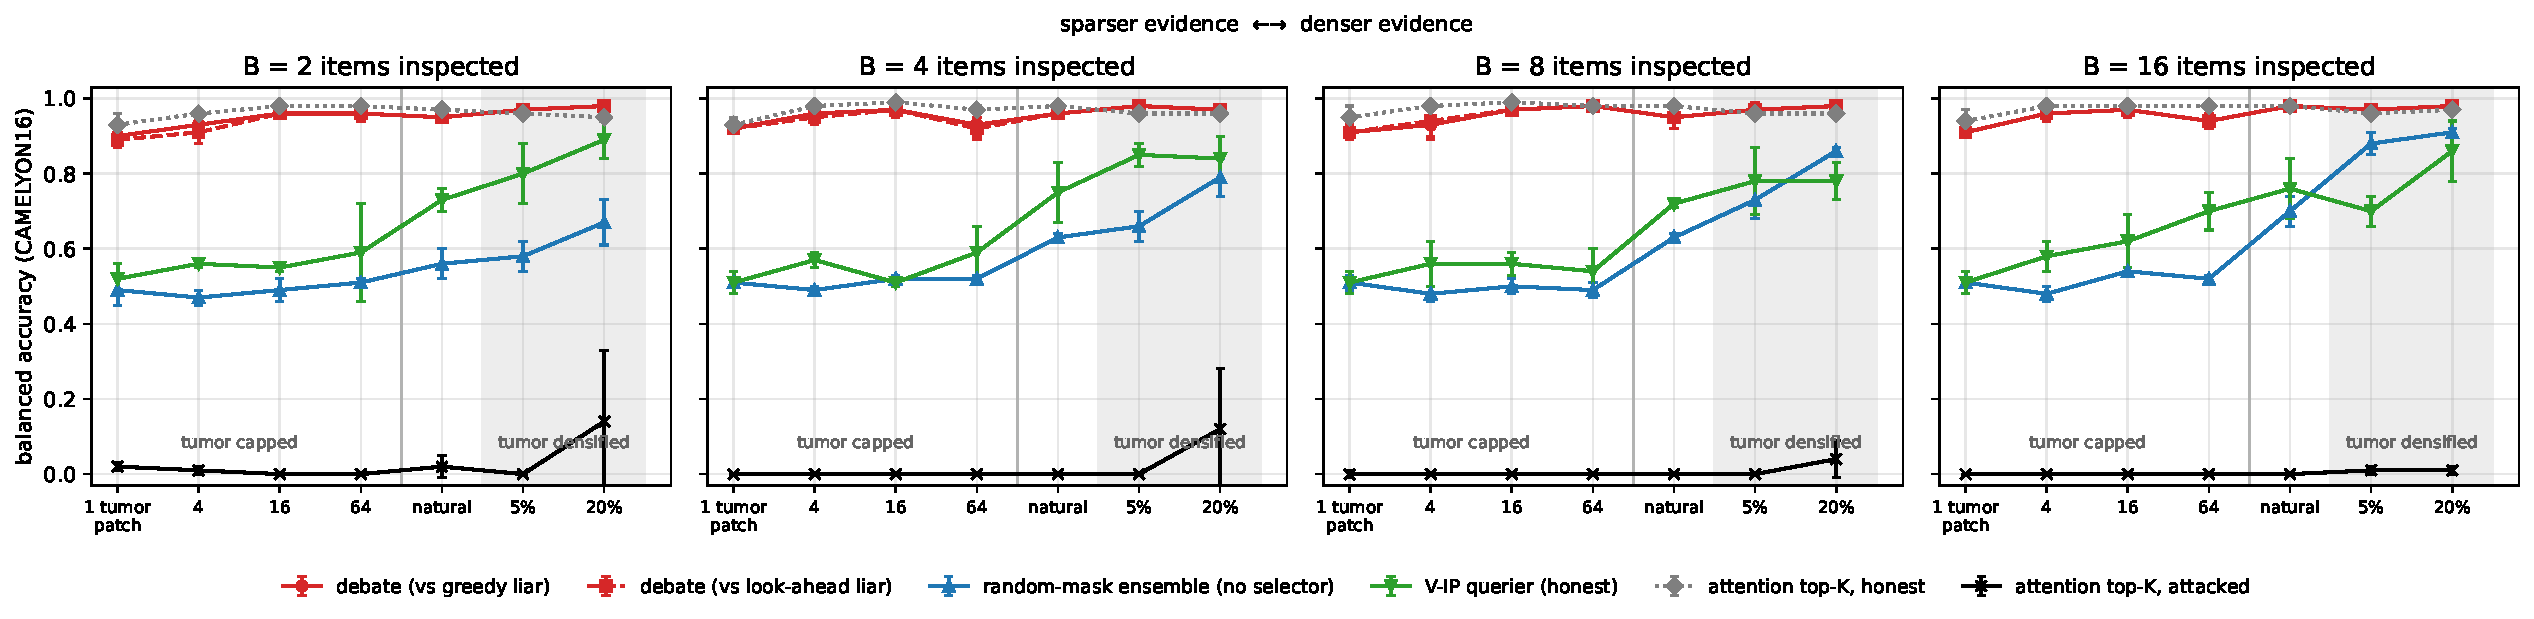
\includegraphics[width=\linewidth]{figs/fig_sparsity.pdf}
\caption{\textbf{Accuracy vs.\ evidence sparsity} (CAMELYON16, 3 seeds; judges retrained per regime; panel title = budget $B$). Left: tumor capped to 1--64 patches (other tumor patches and their neighbours dropped); right: tumor densified to 5\%/20\%. Debate (red) stays at .90--.98 against greedy and look-ahead attackers; random masking (blue) is robust but accurate only when evidence is dense; cooperative selectors (grey, green) collapse under attack (black).}\label{fig:sparsity}
\end{figure*}

\paragraph{Debate under sparsity.} Debate is the only protocol in Fig.~\ref{fig:sparsity} that is both accurate and robust to the specified attackers at every sparsity level. At $B{=}16$, random masking rises from .51 (one tumor patch) to .70 (natural) and .91 (20\% tumor), while debate stays at .91--.98. A judge trained only on random subsets never sees a tumor patch at extreme sparsity, and debate then fails (cap1, $B{=}4$: .67); warm-starting the judge on attention-selected subsets with random presenter flags fixes this (.92) without changing test-time play.

\begin{table}[t]\centering\small
\caption{\textbf{Which ingredient matters?} CAMELYON16 BA (mean$\pm$sd, 3 seeds), every protocol with its own on-policy judge from the same warm start, equal budget $B$. Static: each side selects $B/2$ items for its label without seeing the other side.}\label{tab:mech}
\setlength{\tabcolsep}{3pt}
\resizebox{\linewidth}{!}{\begin{tabular}{@{}lccc@{}}\toprule
protocol ($B$) & 2 & 4 & 8\\\midrule
alternating debate (flags) & .961{\tiny$\pm$.023} & .970{\tiny$\pm$.015} & .957{\tiny$\pm$.011}\\
static counter-selection, flags & .943{\tiny$\pm$.007} & .943{\tiny$\pm$.010} & .927{\tiny$\pm$.018}\\
static counter-selection, no flags & .954{\tiny$\pm$.005} & .962{\tiny$\pm$.011} & .949{\tiny$\pm$.025}\\\midrule
two cooperative readers & .960{\tiny$\pm$.009} & .962{\tiny$\pm$.013} & .975{\tiny$\pm$.015}\\
\ \ one reader compromised & .365{\tiny$\pm$.077} & .289{\tiny$\pm$.071} & .600{\tiny$\pm$.101}\\\midrule
attention top-$B$, attacked & .021 & .000 & .000\\
random masking (32 draws) & .556 & .628 & .628\\\bottomrule
\end{tabular}}\end{table}
\paragraph{Which ingredient matters?} Tab.~\ref{tab:mech}. Removing alternation costs at most 1--3 points, and removing presenter identity does not hurt (static without flags: .949--.962 vs.\ debate .957--.970). Two independent readers are as accurate when both cooperate, but one compromised reader drives them to .29--.60. The effective ingredient is therefore \emph{class-conditioned counter-selection}: a student searches for evidence for each label, so the true label is always represented whichever student is the devil's advocate. Interactive rebuttal is unnecessary in this binary, single-witness setting. When the devil's advocate wins a tumor slide under debate, it is roughly as often because the honest side's witness was outweighed (3--6\% of tumor slides) as because no witness was found (1--3\%).

\paragraph{Can the teacher's doubt replace the second student?} A teacher could instead ask for more evidence whenever it is unsure. We simulate this on CAMELYON16: the teacher starts at $B{=}2$ and escalates to $4$, $8$ and $16$ while its $|\text{logit}|<3$ (each budget with its own on-policy judge; Tab.~\ref{tab:ask}). With two students, escalation is rarely triggered because debate is already near its ceiling at $B{=}2$. With a single adversarial consultant, or attention top-$B$ under attack, the teacher is shown clean normal tissue, is \emph{confidently} wrong, and almost never asks: the escalation leaves BA at 0.00. A teacher cannot be uncertain about a lesion it was never shown; omission is visible only to an opposing student.
\begin{table}[t]\centering\small
\caption{\textbf{Uncertainty-triggered teacher} (CAMELYON16, 3 seeds). Escalate: start at $B{=}2$, request more items while $|\text{logit}|<3$, up to $B{=}16$. avg $B$ = mean items inspected.}\label{tab:ask}
\setlength{\tabcolsep}{3pt}
\begin{tabular}{@{}lcccc@{}}\toprule
 & $B{=}2$ & $B{=}16$ & escalate & avg $B$\\\midrule
two students (debate) & .943 & .958 & .957 & 2.1\\
\ \ look-ahead advocate & .943 & .954 & .954 & 2.1\\
single adv.\ consultant & .000 & .000 & .000 & 2.4\\
attn top-$B$, attacked & .021 & .000 & .000 & 2.4\\
random (one draw) & .532 & .662 & .554 & 3.6\\\bottomrule
\end{tabular}\end{table}

\paragraph{Is it sparsity?} The per-regime results retrain judges and change bag size. \begin{table}[t]\centering\small
\caption{\textbf{Fixed-judge sparsity grid} (CAMELYON16, $B{=}8$, judges trained on natural bags only; 3 seeds). Test tumor slides keep $t$ witnesses; all test slides are subsampled to $N$ patches. Cells: debate / random masking BA, and $p$ = probability that $B$ uniform draws contain a witness, $1-\binom{N-t}{B}/\binom{N}{B}$ (median slide).}\label{tab:sparsity}
\setlength{\tabcolsep}{2.2pt}
\begin{tabular}{@{}lcccc@{}}\toprule
$t\backslash N$ & 256 & 1024 & 4096 & full ($\sim$7.3k)\\\midrule
1 & .79/.51 {\tiny$p$.03} & .85/.50 {\tiny$p$.01} & .84/.49 {\tiny$p$.00} & .88/.50 {\tiny$p$.00}\\
4 & .93/.52 {\tiny$p$.11} & .93/.51 {\tiny$p$.03} & .95/.51 {\tiny$p$.01} & .94/.52 {\tiny$p$.01}\\
16 & .96/.67 {\tiny$p$.29} & .95/.53 {\tiny$p$.08} & .96/.50 {\tiny$p$.02} & .96/.49 {\tiny$p$.01}\\
all (27) & .97/.77 {\tiny$p$.58} & .96/.73 {\tiny$p$.44} & .96/.66 {\tiny$p$.30} & .96/.62 {\tiny$p$.23}\\\bottomrule
\end{tabular}\end{table}
Tab.~\ref{tab:sparsity} separates witness count from bag size under fixed judges. Random masking is at chance whenever $p$ is small and rises with $p$ (.62$\to$.77 as $p$ goes .23$\to$.58), as the uniform-sampling baseline predicts. Competing acquisition depends on the witness \emph{count} and hardly on bag size: one witness gives .79--.88, four give .93--.95, sixteen give .95--.96, for every $N$. Its advantage over selector-free reading is thus the expected acquisition advantage of a reader that finds witnesses; what the protocol adds is that this advantage survives a devil's advocate, which attention top-$B$ (0.00 at every cell) and cooperative pairs (Tab.~\ref{tab:mech}) do not.

\begin{figure*}[t]\centering
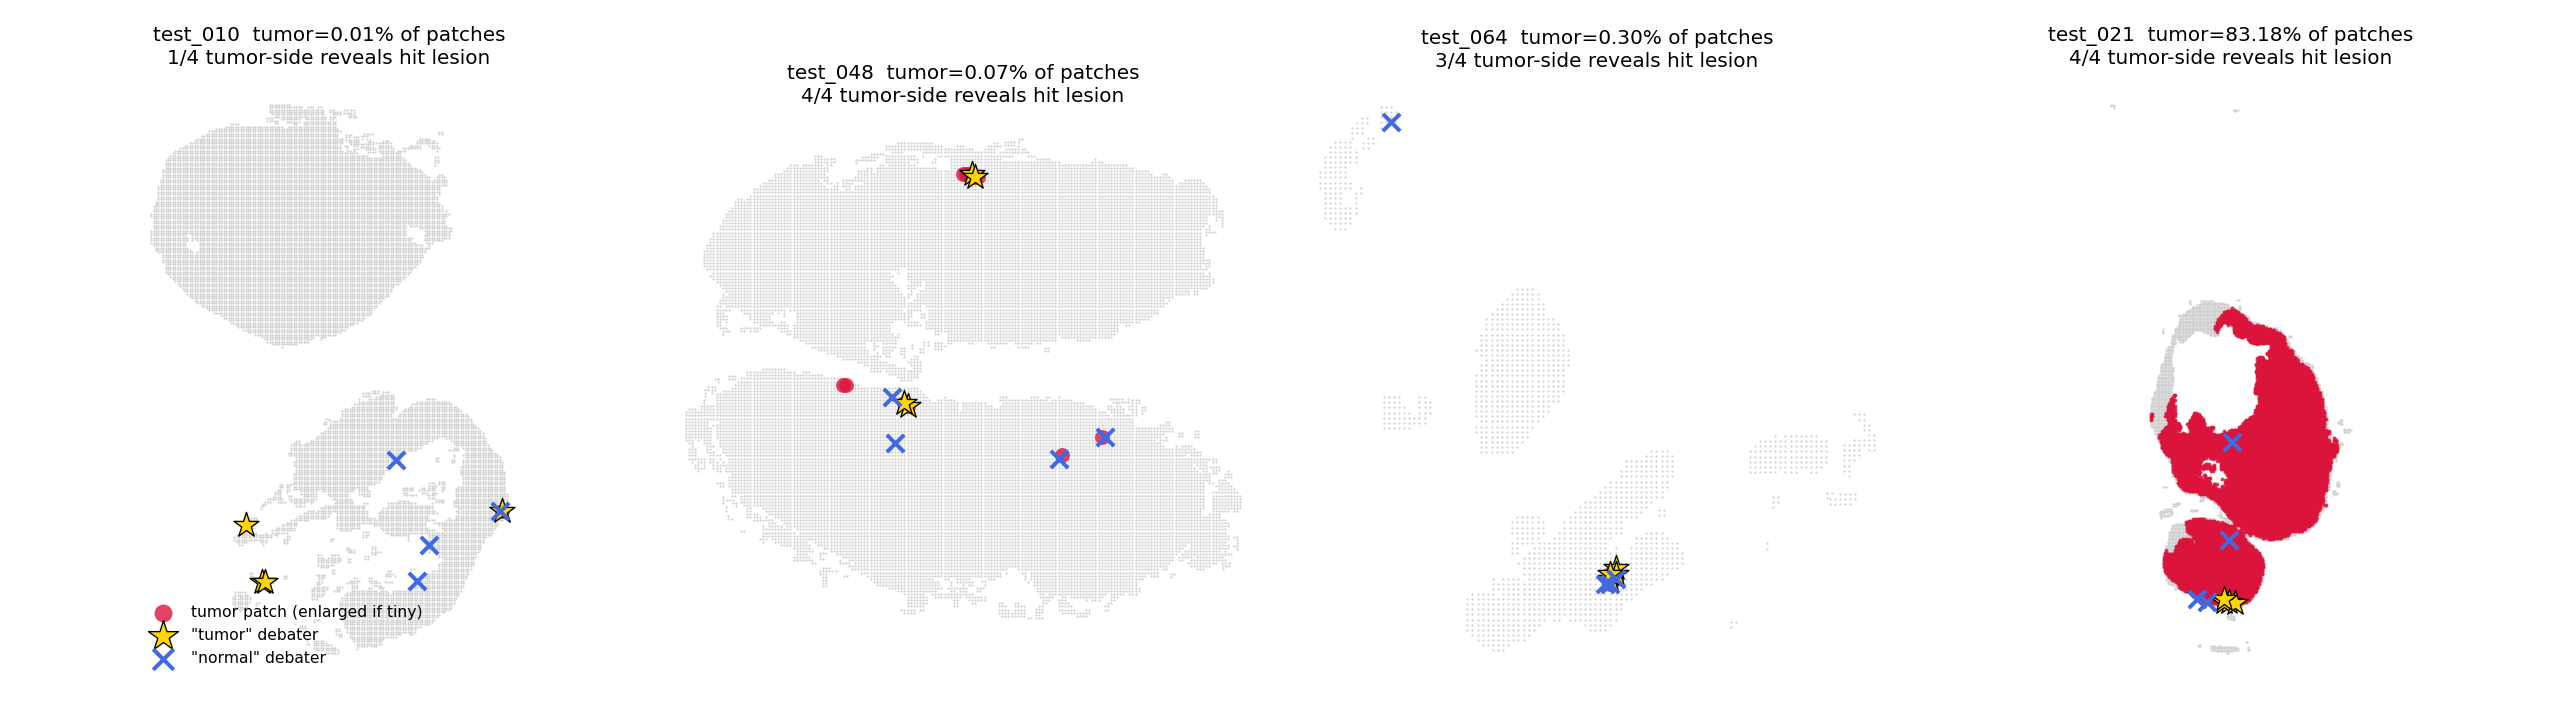
\includegraphics[width=\linewidth]{figs/fig_c16_debate.png}
\caption{\textbf{Debate transcripts on CAMELYON16 test slides} ($B{=}8$). Grey: tissue patches; red: annotated tumor patches (enlarged when tiny); stars: items revealed by the tumor advocate; crosses: items revealed by the normal advocate. Even at 0.01--0.07\% tumor, the tumor advocate reaches lesion patches the normal advocate cannot hide, which is what the judge needs at this budget.}\label{fig:qual}
\end{figure*}

\begin{table}[t]\centering\small
\caption{\textbf{Second encoder} (CAMELYON16, ResNet50 Barlow-Twins features on the same patches; BA mean$\pm$sd, 3 seeds). Full-slide ABMIL: .93 / .50 / .53 per seed.}\label{tab:r50}
\setlength{\tabcolsep}{3pt}
\resizebox{\linewidth}{!}{\begin{tabular}{@{}lccccc@{}}\toprule
$B$ & attn & attn (att.) & cons. (att.) & rand-mask & teaching round\\\midrule
2  & .78{\tiny$\pm$.22} & .30{\tiny$\pm$.21} & .27{\tiny$\pm$.15} & .52{\tiny$\pm$.04} & \textbf{.92}{\tiny$\pm$.04}\\
4  & .75{\tiny$\pm$.24} & .24{\tiny$\pm$.18} & .12{\tiny$\pm$.09} & .51{\tiny$\pm$.09} & \textbf{.92}{\tiny$\pm$.02}\\
8  & .79{\tiny$\pm$.15} & .14{\tiny$\pm$.14} & .29{\tiny$\pm$.16} & .60{\tiny$\pm$.02} & \textbf{.91}{\tiny$\pm$.06}\\
16 & .79{\tiny$\pm$.14} & .09{\tiny$\pm$.07} & .45{\tiny$\pm$.03} & .64{\tiny$\pm$.07} & \textbf{.95}{\tiny$\pm$.01}\\\bottomrule
\end{tabular}}\end{table}
\paragraph{Second encoder.} With ResNet50 Barlow-Twins features (Tab.~\ref{tab:r50}), the selection attack still drives attention top-$B$ to .09--.30 and a single adversarial consultant to .12--.45, while the teaching round (debate) keeps .91--.95 at every budget against greedy and look-ahead devil's advocates; static counter-selection gives .89--.94 and two readers with one compromised .56--.63. With these weaker features, full-slide and attention top-$B$ ABMIL training is unstable across seeds (full-slide .93/.50/.53), whereas teachers trained on presented items stay within .82--.97 on every seed.

\paragraph{Judge controls.} Judges trained from scratch on debate transcripts agree (.95--.97); blank patches with real flags give exactly .500; the devil's advocate wins mostly by hiding (4--10\% of tumor slides at $B{=}4$--8) rather than by making normal tissue look like tumor (1--2.5\% of normal slides). A reader that does not search (random honest side) loses (.14--.53): the protocol requires a competent reader, and correlated omissions by both readers are outside what it can repair.

\paragraph{Diffuse labels.} On BCNB, competing acquisition does not beat random masking (ER .743 vs .731, PR .721 vs .736, Grade-3 .711 vs .724, $B{=}8$). Consistent with Fig.~\ref{fig:sparsity}, its value appears where single witnesses are decisive; we do not claim BCNB labels are uniformly readable from every region.

\paragraph{VLM, label-free.} \begin{table}[t]\centering\small
\caption{\textbf{Label-free VLM advocacy} (accuracy, 95\% CI; global view always shown). $n$ = number of options (2 or 4). Advocates and attackers choose among the same grid tiles using the judge's option scores.}\label{tab:vlmdeb}
\setlength{\tabcolsep}{2pt}
\resizebox{\linewidth}{!}{\begin{tabular}{@{}lccc@{}}\toprule
 & V* Qwen2.5 & V* Qwen3 & HR-4K Qwen2.5\\\midrule
cooperative, 2 crops & .806 {\tiny[.75,.86]} & .901 {\tiny[.85,.94]} & .690 {\tiny[.63,.76]}\\
cooperative, $n$ crops & .812 {\tiny[.75,.86]} & .911 {\tiny[.87,.95]} & .690 {\tiny[.63,.76]}\\
attacked, 2 crops & .356 {\tiny[.29,.42]} & .325 {\tiny[.26,.39]} & .380 {\tiny[.32,.45]}\\
attacked, $n$ crops & .366 {\tiny[.29,.44]} & .335 {\tiny[.27,.40]} & .390 {\tiny[.32,.46]}\\\midrule
\textbf{advocate per option} ($n$ crops) & \textbf{.806} {\tiny[.75,.86]} & \textbf{.843} {\tiny[.79,.90]} & \textbf{.705} {\tiny[.64,.77]}\\
top-2 options advocate (2 crops) & .691 & .780 & .675\\
\ \ truth among top-2 & .859 & .901 & .815\\\bottomrule
\end{tabular}}\end{table}
Tab.~\ref{tab:vlmdeb}. Without any label, giving every option an advocate that shows its best-supporting tile keeps accuracy at .806/.843/.705 although $n{-}1$ advocates are devil's advocates for wrong answers. This matches honest cooperative selection at the same crop budget on V* Qwen2.5 and HR-Bench, and costs 7 points on Qwen3, whereas an attacker controlling the same number of crops drives accuracy to .33--.39. Restricting advocacy to the two answers most likely under the global view is weaker, because the truth is outside that pair for 10--19\% of questions: the competing-acquisition guarantee needs every candidate answer represented. An earlier oracle variant that assigned the honest side the ground-truth option (.78/.83/.70) is not used for claims.

%=====================================================================
\section{Discussion and limitations}\label{sec:discussion}
\textbf{Scope of robustness.} Greedy, look-ahead and RL-trained attackers lose against competing acquisition in our settings; this is empirical robustness to those attackers, not a worst-case guarantee. A few authentic normal patches cannot certify the \emph{absence} of a lesion: without a competent reader that searches the whole slide, two slides can yield the same normal views. \textbf{Compute.} Our students score every item; at equal total compute debate ties full-slide MIL (.94--.97 vs .97). The setting is a judge (a clinician, an expensive model, a regulator) that can inspect only $B$ items chosen by untrusted students, as the senior physician in a case conference does. \textbf{Teacher questions.} Our teacher does not query the students; an interactive teacher that asks targeted follow-ups (rebut a presented region, show its context) is the natural extension, and Tab.~\ref{tab:ask} shows that its questions must be directed at an opposing student rather than triggered by its own doubt. \textbf{Coverage.} Two encoders on CAMELYON16 and one on BCNB; no WSI agent (e.g.\ GIANT, PathFinder) is audited in its native workflow yet; VQA uses one run per question with bootstrap CIs.

\section{Conclusion}
Selected-evidence pipelines inherit the reliability of their selector, in three distinct ways: MIL decisions can be omitted or overridden by authentic evidence, VLM zoom is useful precisely because it is evidence-dependent and therefore steerable, and an RL-trained agent can be robust only because it ignores its own tool. Competing evidence acquisition keeps a budget-restricted judge accurate where single witnesses decide, which is where selection is needed most.

{\small\bibliographystyle{ieeenat_fullname}\bibliography{refs}}
\end{document}
